\chapter{Design and Implementation} %  Design Principles and Architecture
% - 5-10 pages
% - goal: fellow student understands content and would be able to more or less reproduce work
% - legitimate chosen approach
% - develop own ideas, trace them to existing theories
% - analysis and development
% - why was the approach (algorithm/technique/...) chosen and how does it work
% - show how concepts from theory are applied
% - test setup and achieved results

% possible steps:
% - requirement study
% - analysis / design -> UML, interaction, behavioural model, basic algorithms/methods, detailed description of models and their interactions (class/sequence diagrams)
% - manual, how to use program/device
% - system development and implementation

%%%%% start writing here

This chapter is dedicated on the actual implementation details of an orchestration tool that is able to provision bare-metal machines as described by a \gls{dslacr} - more specificaly with \gls{toscaacr} and an extension.
\newline
Overall goals are the ability to understand (parse and interpret) \gls{csaracr} files, to provision bare-metal machines on-demand, and to be compatible with \textquote{normal} (meaning non-bare-metal) provisioning to install applications on the machines.

% considerations:
% - ipv6 not 100 percent necessary, but would be good
% - easy to learn
% - easy to adapt (to counterpart-interface updates) -> plug-in system?
% - tosca-orchestrator:
%   - 4.3ff of \url{http://docs.oasis-open.org/tosca/TOSCA-Instance-Model/v1.0/csd01/TOSCA-Instance-Model-v1.0-csd01.html#_Toc500843787}
%     "orchestrators manage the state of nodes and transitions them from state to state. This notion of state is somewhat artificial in that the orchestrator assumes a stable state is reached after an operation executes [...] without error"
%     "an error results in an undefined state" (no automatic rollback defined in tosca)
%     "orchestration states are only valid during orchestration. [...] the orchestrator or the imperative workflow [...] must decide the current state of all nodes in the topology.
%     "[...] event stream can be maintained for the life of a deployment [...]"
%     "As nodes are transitioned through their states, a subset of attributes and relationships may be defined. [...] This requires that in general TOSCA implies semantics such that not all attributes would be available in a given state."
%     "Nodes are only visible when they have a state defined (i.e. the orchestrator is dealing with their lifecycle)"
%     "node attributes are only defined for the stable states"
%     "node relationships are always navigable when the source and target node exists"
%     "[...] state is never updated outside an orchestration. [...] no way to propagate state changes from the node to the orchestrator and nodes don't have a state attribute."
%       -> no state file!
%     "Nodes can update their attributes with no specific guarantees in terms of precision or accuracy"

\section{Requirements}
The orchestrator should understand \gls{toscaacr}, extensions from it, and should be able to provision bare-metal machines. Not only is it possible to split this into subtasks, but it makes sense as well. By doing so, the modules can be developed and updated one after another, in parallel if necessary and at a later point even interchanged with other implementations. To slice the application into reasonable packages, their domains should not overlap, and their external interface as small as possible.
\newline
To achieve that goal, the application workflow needs to be analyzed:
\newline
In the beginning, the \gls{csaracr} files, its content and the \gls{yamlacr} structure of the content needs to be parsed and validated. This includes handing down properties of both type-from-type and template-from-type derivations, as well as enabling (namespaced) imports.
Then, the orchestrator must be able to wake machines with \gls{wolacr}.
After a machine is powered on, it attempts to boot over the network.
Therefore, the orchestrator has to manipulate an external or internal (as in \textquote{integrated into the orchestration software}) \gls{dhcpacr} server.
To provide the orchestrator with the necessary information about the machine, it makes sense to use a live-\gls{osacr} that does not need to be installed but can be booted directly. Optimally, it should be relatively small, since it is transferred via the network, boot fast, and somehow provide the orchestrator with information about the underlying hardware like its RAM size.
The last step is then running commands like installing a package on or copying files to the machine. Optimally, the user should be informed of what is currently going on during the whole process.
\newline
Figure \ref{image:workflow} shows the whole workflow in an interaction overview diagram.

\begin{figure}[H]
  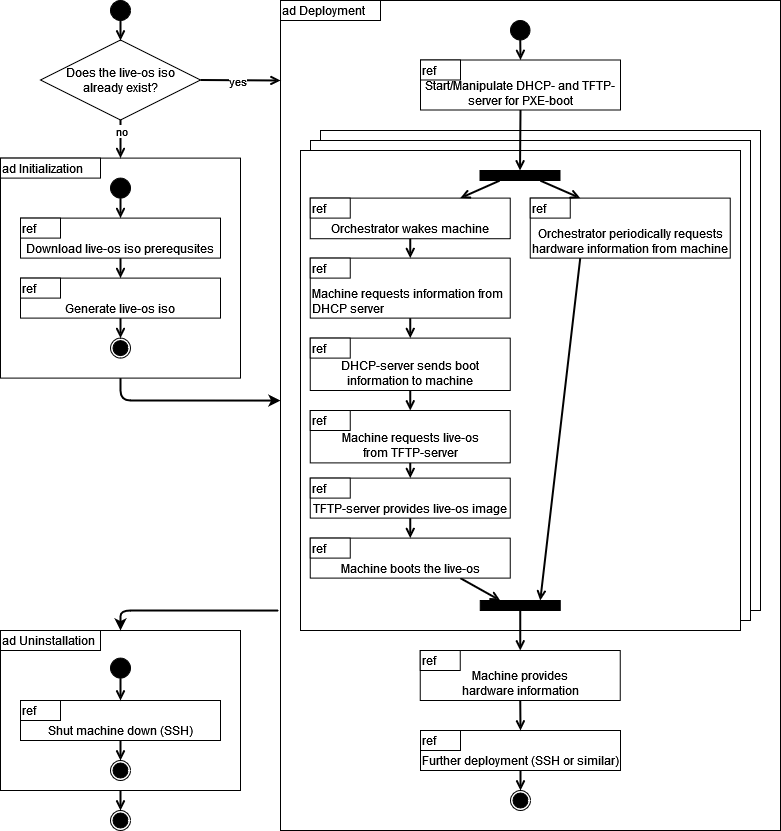
\includegraphics[width=14cm]{workflow}
  \centering
  \caption{UML interaction overview diagram describing the application workflow}
  \label{image:workflow}
\end{figure}

\section{Architecture}
To diminish the limitations of a web-based approach for the orchestrator like the hogging of resources even during idle times, the goal is to have one or many libraries, and a command-line-based wrapper around it.
\newline
As described above, the tasks of the orchestrator can (and should) be split into different steps. For example, the Wake-on-LAN part and the \gls{dhcpacr} server have nothing in common except both being invoked from the orchestrator whenever they are needed.
\newline
The executable has at least three subcommands; One for initialization, where the live-\gls{osacr} image is generated, and the \gls{dhcpacr} server is prepared. And a second where the actual deployment happens. Last but not least, an uninstallation subcommand is needed to reverse the deployment.
\newline
The following chapters describe how the domains within those subcommands are sliced to have different modules for the different domains.

\section{Packages}
Most of the packages described in the following chapters strongly relate to the steps described in figure \ref{image:workflow}. They are described in the order they are invoked during both the initialization and deployment subcommands. A summary of interactions and dependencies is shown in the package diagram in figure \ref{image:packages} below. The most important dependencies are marked with \mintinline[bgcolor=lightgray,breaklines]{bash}{<<use>>}, whereas simple type imports are marked with \mintinline[bgcolor=lightgray,breaklines]{bash}{<<import>>} and have a dashed line.

\begin{figure}[H]
  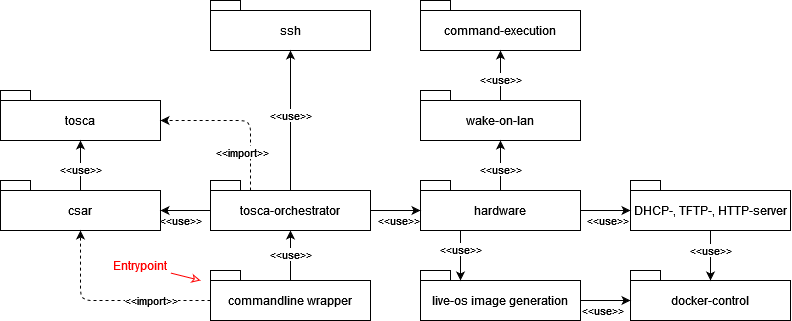
\includegraphics[width=14cm]{packages}
  \centering
  \caption{UML package diagram describing how the packages are related to each other}
  \label{image:packages}
\end{figure}

As can be seen in the diagram, the command-line wrapper communicates only with one package: The orchestrator, which does all of the actual work. For non-bare-metal applications, the orchestrator only uses the \gls{csaracr}, the \gls{sshacr}, and the hardware package directly. The former two are sufficient to be compliant with the current standard specification. When bare-metal machines should be provisioned, the orchestrator also communicates with the hardware package. It manages the generation of the live-\gls{osacr} image, the interactions with the \gls{dhcpacr}-, \gls{tftpacr}-, and \gls{httpacr}-servers, as well as the wake-process of the bare-metal machines.
\newline
When invoked with the initialization subcommand, the application assumes hardware will be provisioned and generates the necessary artifacts.
\newline
Deployment of applications starts with parsing the \gls{csaracr} contents. While the \gls{csaracr} package handles file-I/O, the \gls{toscaacr} package is the actual parser.

\subsection{Commandline-wrapper}
Due to its nature as a wrapper, the sole purpose of this package is the translation of command-line arguments and flags into the correct call to methods of the orchestrator package. The package is also responsible for differentiating between subcommands and additional arguments. During that process, it also validates the mix of arguments and flags.
\newline
This package is the entry point of the whole application, and it translates what the user wants into what the orchestrator understands. Apart from this, its implementation is relatively unspectacular and mostly self-explaining.

\subsection{Orchestrator}
The orchestrator is the center of the application. It is getting called once per execution by the command line wrapper. Afterward, the orchestrator controls what happens during the runtime. In case of a new deployment, the orchestrator will first call the \gls{csaracr} package with the file path of the \gls{csaracr} file. The result is a fully parsed \gls{toscaacr} instance (more on this in the other chapters). Depending on the contents, the orchestrator will execute commands on the local machine, remotely via \gls{sshacr} and/or make calls to the hardware package. Therefore, it is also responsible for conforming to dependencies between the components defined in the \gls{csaracr} file. This includes as much parallelization as possible regarding the steps necessary to reach the desired state.
\newline
The \gls{toscaacr} standard defines several conformance targets. Most of them refer to the files and their structure, two of them are the \gls{toscaacr} processor and the \gls{toscaacr} orchestrator. This package conforms to the latter. This means it contains a processor (the \gls{toscaacr} package described next), can process \gls{csaracr} files (with the \gls{csaracr} package also described later), all \gls{toscaacr}-internal functions defined by the specification and generates meaningful errors when necessary.

\subsection{TOSCA}
To be able to implement a library for the \gls{toscaacr} standard, it is necessary to work through both its actual specification and the Simple-Profile extension counterpart, since both are meant to work together. Important information is sometimes distributed over both specifications, so to fully understand it, both sources are often required.
\newline
Depending on the chosen programming language, such a package might already exist. In the case of this thesis' reference implementation Golang is the language of choice. Sadly, most libraries are either incomplete or based on one another - the most complete of them is severely outdated \cite{github_toscalib_forks}.
\newline
To support the latest version of the \gls{toscaacr} and Simple-Profile specifications, and to be able to easily extend it if necessary, a complete reimplementation of the \gls{toscaacr} library was created. It is strongly influenced by the previously mentioned outdated one but is more complete (and up-to-date). Only with the already described line-by-line read-through of both specifications, it is possible to gather enough information about the standard, how it works, and to differentiate what is contained in the standard and what is just an example.
\newline
With the new library, it is possible to parse any (valid) \gls{toscaacr} Types, Templates, and Service Topologies.
In addition to parsing them and creating Go-native structures out of them, basic functions like \mintinline[bgcolor=lightgray,breaklines]{bash}{get_input} and \mintinline[bgcolor=lightgray,breaklines]{bash}{get_attribute}, it validates that all desired features are implemented. While the specifications were unclear or simply incomplete on several occasions (more on this in the outlook, where possible improvements are discussed), further looks at the reference implementation of OpenTOSCA or the resulting reasonable assumptions helped in creating the library. Some incomplete passages were simply not required for the proof-of-concept this thesis tries to achieve and could therefore be left out during the implementation. The other cases, such as inconsistencies or required assumptions will be covered in the chapter \textquote{Outlook}. %TODO Outlook or Analysis/Discussion?
\newline
Because the basic \gls{toscaacr} specification describes how to work with extensions such as the Simple Profile, it is possible to implement the necessary import-, reference-, and dependency-system as well. This means the implemented \gls{toscaacr} library (called package in Golang context) is fully compatible with the \gls{toscaacr} Simple Profile and all other extensions.
\newline
So, this package does not only parse \gls{yamlacr} to \gls{toscaacr} structures in native Golang but also resolves type derivations, imports, namespacing, and validates them all.
\newline
As described before, this package fulfills the requirements for a \gls{toscaacr} processor. Per the definition, this means it parses and recognizes \gls{toscaacr} elements, generates useful errors when necessary, validates requirements as stated in each type and template definition, resolves imports (while respecting the namespaces), and resolves the defined substitutions.

% TODO describe public functions (all packages)

\subsection{CSAR}
After the \gls{toscaacr} package can parse the contents of files, the file-I/O is implemented as a separate package. The last chapter of the specification (actually in the last chapters of both specifications - the actual standard and the Simple-Profile extension) contains information about how to pack multiple artifacts like \gls{osacr}-images, definition-, or other required files together into one CSAR file. The file is a standard zip archive, but the content needs to follow a certain schema. For example, there are three places where required metadata like version and name can be placed. If they are not found there, the whole file is invalid.
\newline
The reason behind this separation is the still very different domains: The \gls{toscaacr} package parses file contents and provides Go-native types, while the \gls{csaracr} package is more about accessing files, checking for their existence, and making it possible for the \gls{toscaacr} package to parse its content. Should another project work with file contents in a database, for example, they would not require the file handling and can import only the \gls{toscaacr} package.
\newline
This package depends on the earlier described \gls{toscaacr} one, as it has a function that takes a file-/folderpath as input and returns the fully parsed \gls{toscaacr} topology with fully derived templates. \textquote{Fully derived} means that all imports are made and template properties are extended with values from their original type wherever necessary.

%TODO describe public functions

\subsection{Command-execution}
To run Bash commands from the application itself and retrieve the outputs, it makes sense to build a complete package around command execution. It can later be extended with a corresponding implementation for Python, so the application is fully compatible with the \gls{toscaacr} specification.
\newline
The package provides public methods. One for running direct commands, and another for running a script that resides at a provided location.
\newline
Since \gls{toscaacr} only introduces Bash and Python, this package requires the underlying system to be compatible with both script languages. Windows for example does not support Bash by default.

\subsection{Docker control}
Some kind of \gls{dhcpacr}- and \gls{tftpacr}-server is required. They could be external applications, but it should not be a hard requirement. In cases where no external \gls{dhcpacr}- and \gls{tftpacr}-servers exist, it must be possible to set them up in an easily repeatable way. The same applies to the generation of the live-\gls{osacr} image. As in most such cases, this can be solved with (docker) containers. The goal of this thesis is to bring all required bits together, so the application needs to create the docker images, start the containers (with parameters like volumes and forwarded ports), as well as stop and remove the containers when they are not needed anymore (for example when the provisioning is finished).
\newline
The official docker binary (for Linux) is created in Golang as well, and the software is open source. Docker even provides an SDK for other developers to integrate the communication with the docker engine into their applications.
Sadly, the documentation is sparse and the few examples shown along the SDK are often not enough to get even seemingly easy things like container stopping to work. For this case, in particular, it is necessary to add the container (stopping and) removal twice: Once, when the application terminates successfully, as the container fulfilled its job and isn't needed anymore. And a second time, when the application terminates due to an error somewhere else and the default termination is not reached. Even \textquote{deferring} the container termination does not work. Only when the SIGTERM interrupt of the wrapper application is \textquote{manually} listened for and a function removes the container in such a case, the removal is successful in all cases.
\newline
Another obstacle is the retrieval of live logs during the container LiveCycle and embedding the retrieved output in the logs of the wrapping application. This can be solved by creating a buffered stream reader, which is periodically polled and checked for contained linebreaks.
\newline
As the application is now able to handle docker containers to provide repeatable setup of the DHCP- and TFTP-server, the next step is to implement a repeatable way of a live-\gls{osacr} image generation.

\subsection{Live-OS image generation}
The huge amount of time needed to install a complete \gls{osacr} just for retrieving information about the hardware has the potential to be a huge showstopper. To reduce the time needed for information retrieval, a live operating system is used. These operating systems are not necessarily very different from normal ones, but they can most often run from read-only mediums like optical disks. Examples are all \gls{osacr} installers (that can be burned to CD-ROM or similar) - this means there already are many live systems out there.
\newline
Since the live-\gls{osacr} is provided via a network, a virtual version of such a system is required. One such file format for disk images is defined by the ISO 9660 standard \cite{iso9660_spec}. The extension of these files is either \mintinline[bgcolor=lightgray,breaklines]{bash}{.iso} or \mintinline[bgcolor=lightgray,breaklines]{bash}{.udf}. Due to the name of both the standard and the extension, these files are often simply called ISO files.
\newline
To be able to create an ISO file that provides information about the underlying hardware from scratch, only one requirement should exist: A working internet connection. Optimally, a generic preexisting live image is downloaded and then modified to serve the special use case of publishing the desired information. Since tiny Linux images should be relatively common in times of Internet-of-Things and Raspberry Pis, this should be an easy task. The experience tells a different story, though.
\newline
The first Linux distribution tested during the implementation phase was \textquote{Minimal Linux Live}. It is described as an educational Linux, so its configuration is well-documented \cite{mll}. A first test with the original downloaded iso file seemed promising: The file size is less than 50 MB, the \gls{osacr} boots in under 30 seconds and due to its educational background, it is easily extensible. When the system is fully up and running, the keyboard (mouse is not supported) input did not work under the tested Hyper-V hypervisor. As this is not exactly necessary, the image generation was extended in such a way, that a web server is started when the system boots. But with or without this extension, the generated image is not bootable on the said hypervisor. Tested were both the \gls{biosacr} and \gls{uefiacr} firmwares - to no avail.
\newline
A second promising \gls{osacr} is Alpine Linux. It is a full-blown operating system with a focus on a small footprint and a fast boot process. Due to its focus, it is very widespread in the container world, and its documentation is extremely good. There is even a dedicated wiki page for custom ISO-images \cite{alpine_custom_iso}. Since there are additional applications necessary to be installed to generate the image, and these applications are installed with the Alpine Linux package management tool \textquote{apk}, the first test was run in an Alpine-docker-container. Later, the same things were tested with an Alpine-\gls{vmacr}, with the same result. The generated ISO image is four times the size of the original downloadable alpine iso. Not only is there a huge size difference, but when trying to boot it, a kernel file is not found. As described earlier, the overall documentation is quite good, and there are several predefined build profiles for custom images. While the size is different for each one, the kernel file issue reoccurs in all cases. Even when inserting the missing file from the original Alpine iso, the generated iso remains unbootable.
\newline
Another Linux distribution with good documentation and widespread use is Ubuntu. In the Ubuntu app store, there exists a complete graphical application dedicated to image generation. It works perfectly, and the concept with an autostarted webserver that serves information about the underlying hardware can be considered proven. But since the size of the iso file exceeds one GB, and the boot time is close to one minute, another well-known operating system was tried.
\newline
Due to slower release cycles, Debian is considered more stable than Ubuntu. At the same time, it does not have as many features (preinstalled). Therefore its initial size is significantly lower and its non-tweaked performance is generally better. While for custom Debian images there is no graphical tool, the Ubuntu one shows the general approach. The steps can be summarized as follows:

\begin{enumerate}
  \item Unpack the original iso file.
  \item Unpack the contained filesystem-image (squashfs).
  \item Simulate a running operating system on the unpacked contents with \mintinline[bgcolor=lightgray,breaklines]{bash}{chroot}.
  \item Make all necessary changes, like installing applications, enabling services, and adding files. This can include boot-menu adjustments like reducing/removing the timeout.
  \item Repack the filesystem-image.
  \item Repack the image with the changed filesystem-image.
\end{enumerate}

The resulting image is smaller than one GB, boots in under ten seconds, is as extensible as the Ubuntu image, and due to its textual nature completely scriptable. Especially the last part makes it the perfect fit for putting it in a container. It is therefore the selected way to generate a live-\gls{osacr} image.
\newline
The customizations include a webserver that autostarts during boot and a simple service that also starts automatically during the boot process. The service runs some commands and stores the output into files that are then served by the webserver. Due to the proof-of-concept nature, only information about the CPU and RAM is served.
\newline
After retrieving information about the hardware, there are two ways to install further applications. One is to go with the live-\gls{osacr}, and just install the necessary applications. The other is to tell the \gls{dhcpacr}- or \gls{httpacr}-server to provide another \gls{osacr} image, which could be configured for unattended installation. The former has the advantage of being a really fast, standardized and low-resource-usage approach. This is also the way how VMware automatically deploys its ESXi hypervisor clusters. The latter has the advantage of being more flexible regarding the \gls{osacr} and its settings.
\newline
To decrease provisioning times as much as possible, to bring hardware closer to the ephemeral nature of containers, as well as to push the idea of treating machines like cattle, this thesis will pursue the former approach and use the live-\gls{osacr} to install and run additional applications.

\subsection{DHCP-, TFTP-, HTTP-server}
The \gls{dhcpacr}-server does not only provide devices with (temporary) IP addresses but additional information about the network as well. Common examples are the subnet mask and the network gateway for routing beyond the current network. But the \gls{dhcpacr}-server can advertise options for network-boot as well. This includes the URL of a boot firmware on a \gls{tftpacr}-server. Since \gls{biosacr} and \gls{uefiacr} require different files there, a condition is required to run on the \gls{dhcpacr}-server. As described earlier, \gls{tftpacr} is not very efficient, and to support \gls{httpacr}, a boot firmware named iPXE is distributed and loaded before the actual operating system. The loaded iPXE will then send another \gls{dhcpacr} request and will as a result begin to load iPXE anew. To escape this loop, the DHCP-server can detect whether the client is iPXE or not. In case it is not, the iPXE firmware for this specific client is provided (as described above). In case it is, a script location is passed. This can be a simple \gls{httpacr} URL. The \gls{httpacr}-server can then dynamically provide the client with special iPXE-instructions and the actual live-\gls{osacr} image.
\newline
The software dnsmasq combines \gls{dhcpacr} and \gls{tftpacr} server (DNS as well, but that is not needed here). To start and stop the servers on-demand and in one go, dnsmasq and a webserver of choice are installed in a container image. When running the container, the host port 67 (UDP) is required for \gls{dhcpacr}-, host port 69 (UDP) for \gls{tftpacr}-, and host port 80 (TCP) for the \gls{httpacr}-server. The previously generated live-\gls{osacr} image is stored locally to reduce the size of the container image and to have it still available for the next provisioning run.
\newline
The approach described so far is for an environment where no active \gls{dhcpacr} server etc. are already up and running. In the case of other scenarios with those services already being deployed, a compatible integration is necessary. This thesis will focus on a proof-of-concept implementation and thus describe a greenfield approach.

\subsection{Wake-on-lan}
To wake a machine, a so-called magic packet is broadcasted. This packet has a very special format. The only \textquote{real} payload is the MAC-address of the \gls{nicacr} that can power the attached machine when the packet is received.
\newline
This package contains methods for the creation and broadcasting of the magic packet for a MAC address. Since \gls{wolacr} is incompatible with most hypervisors, an additional mechanism has to check whether a hypervisor hosts a \gls{vmacr} with the specified MAC-address. Should this be the case, it determines its identifier and issues the hypervisor to power the \gls{vmacr} on.

\subsection{Hardware}
The hardware package manages the bare metal provisioning process. It controls the container that is responsible for the \gls{dhcpacr}-, \gls{tftpacr}- and \gls{httpacr}-servers. It also initiates the live-\gls{osacr} image generation. Additionally, it issues the calls to the Wake-on-LAN package. Because loading and booting the live-\gls{osacr} takes several seconds, a simple \gls{httpacr} request would time out and the provisioning would fail. Therefore, this package also manages the timeouts and retries until the hardware information is available. Because of the (relatively high - minutes or hours instead of seconds) lease time of issued IP addresses, the \gls{dhcpacr}-server assigns different IP addresses to a machine that wants to boot via the network, and when the live-\gls{osacr} comes up. The hardware package therefore also checks the lease-list of the \gls{dhcpacr}-server for the latest IP address for each MAC address.
\newline
Upon having gathered all desired information about the hardware, the package returns the information to the orchestrator package.
\newline
The orchestrator somehow needs to understand when (and how) to use the hardware package. This is accomplished with an additional \gls{toscaacr} extension similar to the Simple-Profile one. The lowest level node of the standard is the \\
\mintinline[bgcolor=lightgray,breaklines]{bash}{tosca.nodes.Compute} node. It has several attributes like IP addresses and attached networks. Additionally, it provides a capability called \mintinline[bgcolor=lightgray,breaklines]{bash}{tosca.capabilities.Compute}. This capability is required by all \mintinline[bgcolor=lightgray,breaklines]{bash}{tosca.nodes.SoftwareComponent} nodes, which basically means every application that could potentially run on a machine. The \mintinline[bgcolor=lightgray,breaklines]{bash}{Compute} node only requires some kind of block storage. (So, to be accurate, block storage is the lowest level. But in the world of bare-metal, storage requires computing first.)
\newline
In order to be compatible with the original standard as much as possible, an alternative for the \mintinline[bgcolor=lightgray,breaklines]{bash}{Compute} node is defined. This \mintinline[bgcolor=lightgray,breaklines]{bash}{baremetal.nodes.Compute} node provides the exact same capabilities as its \gls{toscaacr} counterpart. Since capabilities are matched via name only, this works seamlessly. In addition, the attributes \mintinline[bgcolor=lightgray,breaklines]{bash}{tosca.nodes.Compute} has, must be available, too. Additional attributes are possible as well, but they are not used by standard \gls{toscaacr} applications. With them, information like desired firmware versions, hardware requirements (like at least two power-supply-units) and more could be defined in the \gls{csaracr} file. 
\newline
In an optimal case, there is a default \gls{osacr}. Then, in order to use bare-metal machines instead of virtual ones, it is sufficient to change the type of the underlying node from \mintinline[bgcolor=lightgray,breaklines]{bash}{tosca.nodes.Compute} to \mintinline[bgcolor=lightgray,breaklines]{bash}{baremetal.nodes.Compute}.
\newline
Currently, the \gls{toscaacr} specification and the Simple-Profile extension do not describe many nodes that could be \textquote{implemented} in hardware. But some examples are \mintinline[bgcolor=lightgray,breaklines]{bash}{tosca.nodes.LoadBalancer} and the aforementioned \mintinline[bgcolor=lightgray,breaklines]{bash}{tosca.nodes.BlockStorage}. Many other devices could and should be supported by this hardware extension, but computing serves well as a proof-of-concept. Routers, switches, or even a \gls{sanacr} are potential candidates for such further \textquote{devices}. Hardware parts are also an option: That way, graphic cards, multiple processors, and multiple \gls{nicacr}s could become node selectors.

\subsection{SSH}
\label{chap:ssh}
%TODO add sources and text on why password auth is bad
To provide the highest possible security for deployed live-\gls{osacr} images, \gls{sshacr} password authentication is disabled. To run remote commands, an \gls{sshacr} public key is included in the image generation workflow. This package manages the generation of a public/private key pair, as well as invoking commands on the remote machines. In the case of the latter, it returns the output to the orchestrator for further processing (like logging). The private key is stored locally next to the infrastructure configuration. The public key on the other hand is embedded in the live-\gls{osacr} images. That way, it is ensured that the communication between orchestrator and machine is secure and that only the orchestrator can invoke commands on it. At the same time, it does not lock access without the orchestrator, so in cases where debugging is necessary, manual \gls{sshacr} access is still possible.
